\documentclass{standalone}
\usepackage{tikz}
\usetikzlibrary{patterns}
\usepackage{siunitx}
\begin{document}
	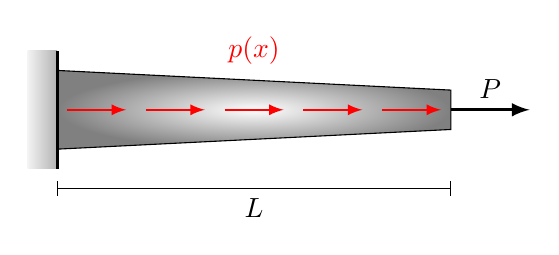
\begin{tikzpicture}[scale=2.5]
		% Barra
		\draw[outer color=gray, inner color=white] (0,-.2) -- (0, .2) -- (2, .1) -- (2, -.1) -- cycle;
		
		% Apoyo
		\shade[left color=gray!10, right color=gray!60] (-.15, -.3) rectangle (0, .3);
		\draw[very thick] (0,-.3) -- (0, .3);
		
		% Acotación
		\draw[|-|] (0, -.4) -- (2, -.4) node[pos=.5, below] {$L$};
		
		% Carga distribuida
		\foreach \x in {0.05, .45, .85, 1.25, 1.65}{
			\draw[-latex, red, thick] (\x, 0) -- (\x + .3, 0);}
		\node[red] at (1, .3) {$p(x)$};
		\draw[-latex, very thick] (2, 0) -- (2.4, 0) node[pos=.5, above]{$P$};
	\end{tikzpicture}
\end{document}